%; whizzy chapter
% -initex iniptex -latex platex -format platex -bibtex jbibtex -fmt fmt
% 以上 whizzytex を使用する場合の設定.

%     Kansai Debian Meeting resources
%     Copyright (C) 2007 Takaya Yamashita
%     Thank you for Tokyo Debian Meeting resources

%     This program is free software; you can redistribute it and/or modify
%     it under the terms of the GNU General Public License as published by
%     the Free Software Foundation; either version 2 of the License, or
%     (at your option) any later version.

%     This program is distributed in the hope that it will be useful,
%     but WITHOUT ANY WARRANTY; without even the implied warranty of
%     MERCHANTABILITY or FITNESS FOR A PARTICULAR PURPOSE.  See the
%     GNU General Public License for more details.

%     You should have received a copy of the GNU General Public License
%     along with this program; if not, write to the Free Software
%     Foundation, Inc., 51 Franklin St, Fifth Floor, Boston, MA  02110-1301 USA

%  preview (shell-command (concat "evince " (replace-regexp-in-string "tex$" "pdf"(buffer-file-name)) "&"))
% 画像ファイルを処理するためには ebb を利用して boundingbox を作成.
%(shell-command "cd image200708; ebb *.png")

%%ここからヘッダ開始.

\documentclass[mingoth,a4paper]{jsarticle}
\usepackage{kansaimonthlyreport}
\usepackage[dvips]{xy}
\usepackage{ascmac}

% 日付を定義する, 毎月変わります.
\newcommand{\debmtgyear}{2011}
\newcommand{\debmtgdate}{27}
\newcommand{\debmtgmonth}{03}
\newcommand{\debmtgnumber}{45}

\begin{document}

\begin{titlepage}

% 毎月変更する部分, 本文の末尾も修正することをわすれずに

 第\debmtgnumber{}回 関西 Debian 勉強会資料

\vspace{2cm}

\begin{center}
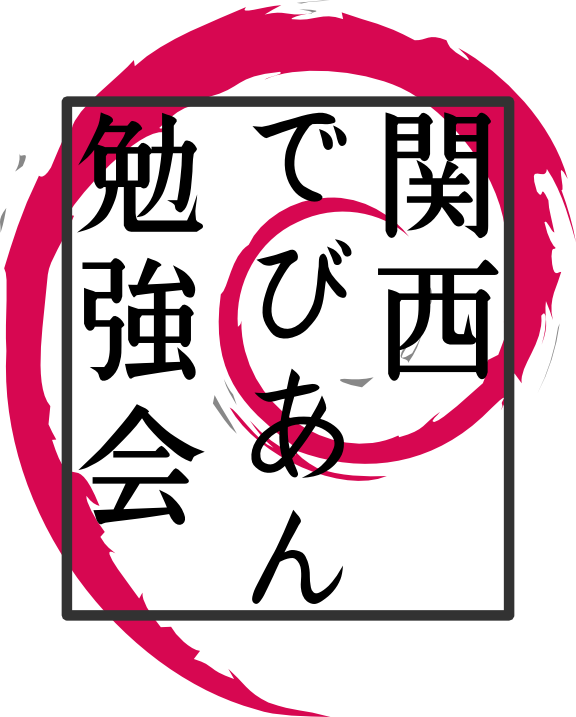
\includegraphics{image200802/kansaidebianlogo.png}
\end{center}

\begin{flushright}
\hfill{}関西 Debian 勉強会担当者 佐々木・倉敷・のがた \\
\hfill{}\debmtgyear{}年\debmtgmonth{}月\debmtgdate{}日
\end{flushright}

\thispagestyle{empty}
\end{titlepage}

\dancersection{Introduction}{Debian JP}

\subsection*{}%ロゴ用のスペース稼ぎ

関西 Debian 勉強会は Debian GNU/Linux のさまざまなトピック (新しいパッケー
ジ, Debian 特有の機能の仕組, Debian 界隈で起こった出来事, などなど) に
ついて話し合う会です.

目的として次の三つを考えています.
\begin{itemize}
      \item ML や掲示板ではなく, 直接顔を合わせる事での情報交換の促進
      \item 定期的に集まれる場所
      \item 資料の作成
\end{itemize}

それでは, 楽しい一時をお楽しみ下さい.

\clearpage

\begin{minipage}[b]{0.2\hsize}
 {\rotatebox{90}{\fontsize{80}{80}
{\gt 関西 Debian 勉強会}}}
\end{minipage}
\begin{minipage}[b]{0.8\hsize}
\hrule
\vspace{2mm}
\hrule
\setcounter{tocdepth}{1}
\tableofcontents
\vspace{2mm}
\hrule
\end{minipage}

\dancersection{最近の Debian 関係のイベント報告}{Debian JP}

\subsection{第 44 回関西 Debian 勉強会}
前回の勉強会は、2 月 27 日に港区民センターでの開催でした。セッションは、
水野さんによる「pbuilder を使ってみよう」と、のがた・倉敷による
「squeeze の変更点をみんなで見てみよう」でした。
pbuilder については、パッケージ作成だけでなく、sid や experimental から
野良バックポートしたい時にも便利ですね。そろそろ squeeze への移行も完了
しているはずですから、前回の配布資料を手元において、是非トライしてみてください。

\subsection{第 74 回東京エリア Debian 勉強会}

東京エリアでは 3 月 5 日に OSC 2010 Tokyo/Spring において、
「第 74 回東京エリア Debian 勉強会」が開催され、
岩松さんによる新安定版 Debian 6.0(Squeeze) と次期バージョン(7.0)へ向けた開発の状況が紹介されました。
また、恒例の GPG/PGPキーサインパーティに加えて
「CAcert サインパーティ」および「日本初! CAcert 公式トレーニング(ATE Tokyo)」も開催されています。
CAcert はユーザが自由に X.509 証明書を持てるようにするプロジェクトです。
東京では 12 月の勉強会で CAcert に関する話題を扱っています%
\footnote{\url{http://tokyodebian.alioth.debian.org/pdf/debianmeetingresume201012.pdf}}。
関西でもそのうち CAcert についての話題を取り上げようと(個人的には)思います。



\clearpage
%-------------------------------------------------------------------------------
\dancersection{Debian のドキュメントをみてみよう}{かわだてつたろう}

\subsection{はじめに}
Debian プロジェクトはユーザに向けたドキュメントを提供しています。ドキュ
メントパッケージを管理する doc-base のクライアントとともに Debian を使っ
ていくうえで有用な Debian 固有のドキュメントをいくつか紹介します。


\subsection{doc-base}
doc-base とは Debian システムにインストールされたドキュメントを管理す
るユーティリティとドキュメントのメタデータのデータベースを提供するパッ
ケージです。単なる man ページだけでなくオンラインドキュメントを提供す
る Debian パッケージはインストール時に doc-base に登録し、アンインストー
ル時に登録を解除することが推奨されています。\footnote{Debian Policy
 Manual: 9.10 Registering Documents using doc-base}
doc-base に登録されたメタデータを利用するクライアントとして dwww,
dhelp, doc-central などが提供されています。これらクライアントを利用す
ればドキュメントの検索、閲覧が容易に行えます。

\subsection{doc-base クライアント}
doc-base クライアントをいくつか紹介します。


\subsubsection{dwww}
dwww はウェブベースのドキュメントリーダです。

doc-base に登録されたドキュメント、man、info を参照することができます。
ドキュメントはインデックス化されており検索することができます。

\subsubsubsection{インストール}

apt を使用してインストールするだけですが info を表示する info2www の設
定が少し必要です。

info2www のシンボリックリンクを作成して info2www をドキュメントルート
下(ここでは /var/www)に公開させます。info2www を公開させなくても動作し
ますが info を表示する場合に画像などが表示されません。
\footnote{/usr/share/doc/info2www/README.Debian 参照}

またインストール直後はインデックスの作成に少し時間がかかりますのでしば
らく待ってから dwww を使用してください。

\begin{commandline}
$ sudo aptitude install dwww
$ sudo ln -s /var/lib/info2www /var/www/info2www
\end{commandline}

\subsubsubsection{使い方}

WEB ブラウザで \url{http://localhost/dwww} にアクセスするかコマンドラ
インで dwww と実行してください。ブラウザに dwww のホームが表示されます。
後は WEB ブラウジングするようにリンクを辿るか入力フォームにキーワード
を入力して検索を行ない目的のドキュメントを探してください。残念ながら日
本語での検索はできません。

検索はコマンドラインから行なうこともできます。例えば debian という検索
をコマンドラインから行ないたい場合は以下のように実行すれば WEB ブラウ
ザに debian と検索した結果が表示されます。

\begin{commandline}
  $ dwww debian
\end{commandline}


\subsubsection{dhelp}
dhelp はウェブベースのドキュメントリーダです。

WEB ブラウザから doc-base に登録されたドキュメントを参照することができ
ます。ドキュメントはインデックス化されており検索することができます。

\subsubsubsection{インストール}

apt を使用してインストールするだけです。dhelp は WEB サーバを必要とし
ていませんのでここで WEB サーバはインストールされません。インストール
直後はインデックスの作成に少し時間がかかりますのでしばらく待ってから
dhelp を使用してください。

\begin{commandline}
  $ sudo aptitude install dhelp
\end{commandline}

\subsubsubsection{使い方}

WEB ブラウザで \url{file://localhost/usr/share/doc/HTML/index.html} に
アクセスするかコマンドラインで dhelp と実行してください。ブラウザに
dhelp のホームが表示されます。後は WEB ブラウジングするようにリンクを
辿ってドキュメントを探してください。この状態では info pages, man pages
の参照、ブラウザからの検索を行なうことはできません。

検索はコマンドラインから行なうことになります。例えば debian という検索
をコマンドラインから行ないたい場合は以下のように実行すれば WEB ブラウ
ザに debian と検索した結果が表示されます。残念ながら日本語での検索はで
きません。

\begin{commandline}
  $ dhelp debian
\end{commandline}

\subsubsubsection{WEB サーバの導入}

WEB サーバを必要としないのは一つのメリットですが制限もあり不便ですので
WEB サーバをインストールして WEB ブラウザからの検索、info と man の参
照ができるようにします。dhelp パッケージが Suggests しているパッケージ
を参考に apache2 と info2www, man2html を追加インストールします。先と
同様に info2www の設定を少し行ないます。

\begin{commandline}
  $ sudo aptitude install apache2 info2www man2html
  $ sudo ln -s /var/lib/info2www /var/www/info2www
\end{commandline}

これで WEB サーバを経由で dhelp を使用できるようになりました。
dhelp コマンドの結果は WEB サーバ経由で表示されるようになりますが WEB
ブラウザに直接アドレスを入力する場合はアドレスを
\url{http://localhost/doc/HTML/index.html} に変更してください。


\subsubsection{doc-central}
doc-central はウェブベースのシンプルなドキュメントリーダです。

WEB ブラウザから doc-base に登録されたドキュメントを参照することができ
ます。doc-central はドキュメントをインデックス化しませんが doc-base の
メタデータに登録されたドキュメント名、作者、概要を対象として検索するこ
とができます。man は参照することができません。

\subsubsubsection{インストール}

apt を使用してインストールするだけですが info2www の設定が少し必要です。

\begin{commandline}
  $ sudo aptitude install doc-central
  $ sudo ln -s /var/lib/info2www /var/www/info2www
\end{commandline}

\subsubsubsection{使い方}

WEB ブラウザで \url{http://localhost/dc/} にアクセスするかコマンドライ
ンで doccentral と実行してください。doc-central ではなく doccentral で
す。ブラウザに Doc-Central のホームが表示されます。後は WEB ブラウジン
グするようにリンクを辿るか入力フォーム\footnote{左側フレームの最下部に
  あります}にキーワードを入力して検索を行ない目的のドキュメントを探し
てください。

検索はコマンドラインから行なうこともできます。例えば debian という検索
をコマンドラインから行ないたい場合は以下のように実行すれば WEB ブラウ
ザに debian と検索した結果が表示されます。

\begin{commandline}
  $ doccentral debian
\end{commandline}


\subsubsection{その他に}

\subsubsubsection{Yelp}

Yelp は Gnome のヘルプブラウザです。

Yelp からは man と info そして Gnome のヘルプが参照できますが各パッケー
ジのドキュメントは参照できません。

\subsubsubsection{khelpcenter}

khelpcenter4 は KDE のヘルプセンタです。

khelpcenter4 からは man と KDE のヘルプが参照できますが info や各パッ
ケージのドキュメントは参照できません。

\newpage

\subsection{The Debian Documention Project のドキュメント}
doc-base クライアントが使えるようになったところで、パッケージとして提
供されている The Debian Documention Project (DDP) のドキュメントをいく
つかざっとみていきます。


\subsubsection{doc-debian}
Debian の基礎となる Debian 社会契約や Debian フリーソフトウェアガイド
ラインといった Debian プロジェクトの基礎となる文書群です。


\subsubsection{installation-guide}
インストールガイドです。

squeeze では 12 種類のアーキテクチャ毎にパッケージが用意されています。
\footnote{squeeze では hppa のサポートが外れ 11 種類のアーキテクチャが
サポート対象ですが installation-guide-hppa パッケージが存在します。}
i386 アーキテクチャ用だとパッケージ名は installation-guide-i386 になり
ます。

初めて Debian をインストールする場合に参照することになるでしょう。
CD-ROM/DVD-ROM や USB メモリといったメディアからのインストール以外にも
debootstrap やネットブートを使用したインストール方法、preseed を利用し
たインストールの自動化についても説明されています。ちょっと違ったインス
トールをする場合にも参考になることが記載されています。

手早くインストールの流れを確認するだけなら「付録 A. インストール Howto」
を参照してください。もしもの場合に供えて「5.4. インストールプロセスの
  トラブルシューティング」も見ておくことをおすすめします。


\subsubsection{debian-reference}
Debian システムの広範な概論です。

日本語訳は debian-reference-ja として別パッケージで提供されています。

内容は大変多岐に渡りコンソールの基礎から Debian でのパッケージ管理、ネッ
トワーク設定、プログラミングまで扱っています。DDP の中でも最も充実した
ユーザマニュアルです。

Unix ライクなシステムを使った経験があまり無いのであればぜひ
「1. GNU/Linux チュートリアル」を参照してください。Debian のパッケージ
については「2. Debian パッケージ管理」で詳細に説明されています。
unstable を使いはじめようという時には「2.6. 壊れたシステムからの復元」
が手助けになるかもしれません。その他 Debian を使っている各局面にあわせ
て項目を参照してみるとよいでしょう。


\subsubsection{maint-guide}
新たにパッケージメンテナになろうという人向けの解説です。

「Debian 新メンテナガイド」、「Debian メンテナ入門」、
「ニューメンテナガイド」、「新規メンテナのためのガイド」などと呼ばれて
います。日本語訳は maint-guide-ja として別パッケージで提供されています。

gentoo パッケージを例にとってパッケージの作成、アップロード、更新手順
が説明されています。
内容の大半がパッケージ作成に割かれて詳しく説明されていますのでパッケー
ジメンテナになろうという人だけでなく、Debian のパッケージを作ってみよ
うと思う方も是非参照してください。


\subsubsection{developers-reference}
Debian 開発者向けのリファレンスです。

日本語訳は developers-reference-ja として提供されていますが翻訳途中で
す。

新規メンテナプロセスから始まり Debian Developer が使用できるリソース、
パッケージの扱い方が説明されています。特に技術的な事柄以外のパッケージ
化についてありとあらゆる情報が記載されています。
Debian Developer の活動の一部を垣間見られるドキュメントです。


\subsubsection{debian-policy}
Debian ポリシーマニュアルとポリシーを補足する文書群です。

Debian ポリシーマニュアルには Debian パッケージの内部構造(アーカイブ構
成、パッケージの各書式など)やオペレーティングシステムとして必要な設計
部(ファイルシステムの階層構造、システムや各種プログラムの設定など)につ
いて記載されています。日々議論され更新されています。

日本語訳されたパッケージはありませんが Debian JP Project で Debian ポ
リシーマニュアル(Version 3.8.3.0)を翻訳したものが WEB で公開されていま
す。
\footnote{\url{http://www.debian.or.jp/community/devel/debian-policy-ja/policy.ja.html/}}
過去に東京エリア Debian 勉強会でとりあげられていますのでその資料も参考
にしてみてください。
\footnote{第 12, 13, 15 回東京エリア Debian 勉強会事前資料参照}


\subsubsection{その他}
\subsubsubsection{debian-faq}
Debian に関する FAQ がまとめられています。


\subsubsubsection{harden-doc}
Debian のセキュリティに関することをまとめたマニュアルです。システムの
セキュリティに関することからプロジェクトのセキュリティ取り組みについて
も記載されています。現在、日本語への翻訳が進められています。


\subsubsubsection{debian-refcard}
いわゆるリファレンスカードです。一枚の紙(A4 裏表)に重要なコマンドの一
覧や参考となる情報をまとめてあります。


\subsection{最後に}

ドキュメントは随時更新されており最新ドキュメントは  Debian のユーザ文
書\footnote{\url{http://www.debian.org/doc/}}にまとめられていますので
確認してみてください。ここにはパッケージになっていないドキュメント(例
えばリリースノートなど)もあります。
ドキュメントソースは Subversion で管理、公開されておりどなたでも確認す
ることができます。興味があればこちらも覗いてみてください。
\footnote{\url{http://www.debian.org/doc/cvs.ja.html}}

ドキュメントに間違いを見つけた場合は BTS するか、日本語訳に関すること
であれば \url{debian-doc@debian.or.jp} に報告するとよいでしょう。

また、The Debian Documention Project が提供するドキュメント以外にもソ
フトウェアのドキュメントパッケージがたくさんありますのでパッケージの
``doc'' セクションも覗いてみてください。

\subsection{参考資料}
\begin{itemize}
 \item Debian ユーザ文書: \url{http://www.debian.org/doc/}
 \item doc-base: \url{http://wiki.debian.org/doc-base/}
\end{itemize}

%-------------------------------------------------------------------------------
% Copyright (C) 2011 Tatsuya Kinoshita
% This work comes with ABSOLUTELY NO WARRANTY.  Unlimited permission is
% granted to use, copy and distribute it, with or without modification,
% either commercially or noncommercially.
\dancersection{「フリー」って、どういうこと?}{木下 達也}
\subsection{フリーソフトウェアとは}

Debianはフリーソフトウェアで構成されたオペレーティングシステムです。
ここで言う「フリー」とは「無料」ではなく「自由」を意味しています。

Free Software Foundation (FSF)による『フリーソフトウェアの定義』
では次のように説明されています。

\begin{quote}
「フリーソフトウェア」のフリーとはそのソフトウェアの
ユーザに与えられる4種類の自由を意味しています。

\begin{itemize}
 \item 目的を問わず、プログラムを実行する自由(第0の自由)。

 \item プログラムがどのように動作しているか研究し、そのプログラムに あなたの必要に応じて修正を加え、採り入れる自由(第1の自由)。ソースコードが入手可能であることはこの前提条件となります。

 \item 身近な人を助けられるよう、コピーを再頒布する自由(第2の自由)。

 \item プログラムを改良し、コミュニティ全体がその恩恵を受けられるよう あなたの改良点を公衆に発表する自由(第3の自由)。ソースコードが入手可能であることはここでも前提条件となります。

\end{itemize}

(\url{http://www.gnu.org/philosophy/free-sw.ja.html})
\end{quote}

\subsection{著作権とライセンス}

著作物には、基本的に著作者に対して著作権が発生しており、
著作物を変更したりコピーして配ったりするには、
著作者からの許可(ライセンス)が必要になります。

フリーかどうかを判定する際には、
変更や配布が許可されているか、
それらに付随する制約はどうか、
といった点を確認します。

そのほかに、特許、商標など個別の事情についても検討します。

\subsection{Debianフリーソフトウェアガイドライン}

ある著作物がフリーかどうか、Debianの構成要素として適しているかどうかを
判定する際の基準、それがDebianフリーソフトウェアガイドライン(DFSG)です。

\begin{quote}
\begin{enumerate}
 \item 自由な再配布

 \item ソースコード

 \item 派生ソフトウェア

 \item 原作者によるソースコードの整合性維持

 \item すべての個人、団体の平等

 \item 目標分野の平等

 \item ライセンスの配布

 \item ライセンスはDebianに限定されない

 \item ライセンスは他のソフトウエアを侵害しない

 \item フリーなライセンスの例

\end{enumerate}

(\url{http://www.debian.org/social_contract#guidelines})
\end{quote}

DFSGの各条項について簡単に説明します。

\begin{enumerate}
 \item 自由な再配布 (Free Redistribution)

有償・無償を問わず、別途の許可を必要とすることなく、
プログラムを複数まとめて配布できます。

 \item ソースコード (Source Code)

ソースコード(変更に適した形式)が必要です。
実行形式だけでなくソースコードでも配布できます。

 \item 派生ソフトウェア (Derived Works)

同様のライセンスで変更版を配布できます。

 \item 原作者によるソースコードの整合性維持
   (Integrity of The Author's Source Code)

変更版のソースコードを配布する場合に、
元のソースコードと差分(パッチ)という形式のみ許可
という制約は許容します。ただし非推奨です。

 \item すべての個人、団体の平等
   (No Discrimination Against Persons or Groups)

いかなる個人・団体も差別せずに許可します。

 \item 目標分野の平等
   (No Discrimination Against Fields of Endeavor)

商用・非商用など、用途を制限しません。

 \item ライセンスの配布
   (Distribution of License)

ライセンスは、再配布されたすべての人々に、
別途の許可を必要とすることなく適用されます。

 \item ライセンスはDebianに限定されない
   (License Must Not Be Specific to Debian)

Debianの一部としてのみの許可ではなく、
他のシステムにも適用できるようにします。

 \item ライセンスは他のソフトウエアを侵害しない
   (License Must Not Contaminate Other Software)

たとえば、同じ媒体で配布されるソフトウエアすべてが
フリーであることを要求しないようにします。

 \item フリーなライセンスの例
   (Example Licenses)

GNU General Public License (GPL), BSD License, Artistic Licenseが
例として挙げられています。

\end{enumerate}

\subsection{オープンソースの定義}

Open Source Initiative (OSI)による『オープンソースの定義』(OSD)は
DFSGを元に作られました。何度か改訂されていますが、
現状でも内容はDFSGとほぼ同等のものです。

ここでは、一見して異なるOSD第10条についてのみ説明します。

\begin{quote}
10. ライセンスは技術中立的でなければならない

(\url{http://opensource.jp/osd/osd-japanese.html})
\end{quote}

たとえば、GUI環境で「同意する」ボタンを押すことが
必須であってはならない、ということになります。
内容としてはDFSG/OSDの第7条に含まれているものとも言えそうですが、
OSDでは、いわゆるクリックラップについて、この条項で特に注意を促しています。

\subsection{コピーレフト}

コピーレフトとは、著作物やその変更版について、
フリーであることを要求するための方法のことです。

GNU GPLは代表的なコピーレフトライセンスです。
GNU GPLで配布されるソフトウェアは、その変更版の配布についてもGNU GPLが適用され、
フリーソフトウェアであり続けます。

著作物全体への適用が「弱い」コピーレフトライセンスもあります。
たとえば、GNU Lesser General Public License (LGPL)で配布されるライブラリは、
リンクするプログラム全体についてはコピーレフトが適用されません。
そのほかに、Mozilla Public License (MPL)、
Eclipse Public License (EPL)、
Common Development and Distribution License (CDDL)など、
ファイル・モジュール単位でのコピーレフトライセンスもあります。

\subsection{ライセンスの互換性}

複数の著作物を組み合わせて一つの著作物にする場合、
それぞれのライセンスによる要求が矛盾しないかどうか、
互換性が問題になることがあります。

たとえば、CDDLではGNU GPLとは違った要求をしているので、
GNU GPLで配布されるソフトウェアとCDDLで配布されるソフトウェアを
組み合わせた著作物は配布できません。

ライセンスの非互換を回避するには、
複数のライセンスを適用する(デュアルライセンス)、
例外条項を設ける、
単純で何でも許可するようなライセンスにする、
といった方法があります。

\subsection{ASPループホール}

GNU GPLには、アプリケーションサービスプロバイダ(ASP)の
抜け穴(loophole)が存在することが知られています。

手元のコンピュータではなく「あちら側」のコンピュータで
実行されるウェブアプリケーションの場合、
そのウェブアプリケーションがGNU GPLで配布された
ソフトウェアを含んでいたとしても、
ネットワークユーザーにソースコード込みで再配布
されるわけではありません。

その抜け穴をふさぐためのライセンスが
GNU Affero General Public License (AGPL)です。
ネットワークユーザーへのソースコード提供を求める条文が
GNU GPLに加えられたものになっています。

\subsection{自由と協力}

なぜソフトウェアをフリーにするのでしょうか。
フリーソフトウェア、オープンソースの関係者それぞれに様々な思惑があることと思いますが、
ここでは一つの考えを挙げておきます。

個人の自由を促進し人々が協力し合うこと、
自分のためにみんなのために実践できること、
それがソフトウェアに関することなのであれば、
フリーソフトウェアがよく似合います。

Debianプロジェクトはフリーソフトウェアを強く支持しています。

Happy Hacking!

\newpage
\subsection{参考資料}

\begin{itemize}
 \item フリーとは何だろう? あるいはフリーソフトウェアとは何を意味するのか?

\url{http://www.debian.org/intro/free.ja.html}

\url{http://www.debian.org/intro/free.en.html}

 \item フリーソフトウェアの定義

\url{http://www.gnu.org/philosophy/free-sw.ja.html}

\url{http://www.gnu.org/philosophy/free-sw.html}

 \item Debian 社会契約 / Debian フリーソフトウェアガイドライン (DFSG)

\url{http://www.debian.org/social_contract.ja.html}

\url{http://www.debian.org/social_contract.en.html}

 \item Debian -- ライセンス情報

\url{http://www.debian.org/legal/licenses/index.ja.html}

\url{http://www.debian.org/legal/licenses/index.en.html}

 \item DFSG and Software License FAQ (Draft)

\url{http://people.debian.org/~bap/dfsg-faq.html}

 \item オープンソースの定義

\url{http://opensource.jp/osd/osd-japanese.html}

\url{http://opensource.org/docs/osd}

 \item Open Source Licenses

\url{http://opensource.org/licenses/index.html}

 \item コピーレフトって何?

\url{http://www.gnu.org/copyleft/copyleft.ja.html}

\url{http://www.gnu.org/copyleft/copyleft.html}

 \item さまざまなライセンスとそれらについての解説

\url{http://www.gnu.org/licenses/license-list.ja.html}

\url{http://www.gnu.org/licenses/license-list.html}

 \item GNU GPLに関して良く聞かれる質問

\url{http://www.gnu.org/licenses/gpl-faq.ja.html}

\url{http://www.gnu.org/licenses/gpl-faq.html}

 \item Debian について

\url{http://www.debian.org/intro/about.ja.html}

\url{http://www.debian.org/intro/about.en.html}

\end{itemize}

%-------------------------------------------------------------------------------
\dancersection{今後の予定}{Debian JP}

\subsection{4 月神戸 IT フェスティバル + オープンソースカンファレンス 2011Kansai@Kobe}

4 月 15 日 (金)、 16 日 (土) に JR 神戸駅すぐの神戸市産業振興センターにて、 神戸 IT フェ
スティバル + オープンソースカンファレンス 2011Kansai@Kobe が開催されます。

セッションは「第46回関西Debian勉強会  - 遂にリリースされた(?) Squeeze について - 」
で、講演者は佐々木、内容は
「リリースされたDebian安定版 6.0(Squeeze)の紹介とDebian界隈の話題などについてお話しします。」です。
ブースでは、毎度お馴染「Deb専」の販売(と、できれば実機の展示)を行なう予定です。
\begin{center}
  {\bf{ブース要員が足りないので協力して下さる方大歓迎です}}。
\end{center}

また、そろそろ恒例(?)になりつつある GPG キーサインパーティですが、
今回はセッションとして「GPG/PGP の入門」を計画しています(ので、キーサイン自体は別途個々人でお願いします)
\footnote{あと、キーサインパーティの宣伝のために LT に申し込んでみました(佐々木)。}。

以上、皆様新年度もよろしくお願いします。

% 冊子にするために, 4 の倍数にする必要がある.
% そのための調整
\dancersection{メモ}{}
\mbox{}\newpage

\printindex
 \cleartooddpage

 \begin{minipage}[b]{0.2\hsize}
  \rotatebox{90}{\fontsize{80}{80} {\gt 関西 Debian 勉強会} }
 \end{minipage}
 \begin{minipage}[b]{0.8\hsize}

 \vspace*{15cm}
 \rule{\hsize}{1mm}
 \vspace{2mm}
 
\includegraphics[width=2cm]{image200502/openlogo-nd.eps}
 \noindent \Large \bf Debian 勉強会資料\\ \\
 \noindent \normalfont \debmtgyear{}年\debmtgmonth{}月\debmtgdate{}日 \hspace{5mm}  初版第 1 刷発行\\
 \noindent \normalfont 関西 Debian 勉強会 (編集・印刷・発行)\\
 \rule{\hsize}{1mm}
 \end{minipage}

\end{document}
